\documentclass[10pt]{article}
\usepackage[margin=1in]{geometry} 

\usepackage{amsmath,amsthm,amssymb,graphicx,amsfonts}

\usepackage{float}
\usepackage{caption,subcaption} % para las figuras
\usepackage{wrapfig}

\usepackage{comment}

\usepackage[utf8]{inputenc} %tildes
\usepackage[spanish]{babel}

\usepackage{enumerate}

\usepackage{color}   %May be necessary if you want to color links
\usepackage[hyphens]{url}
\usepackage[hidelinks]{hyperref}
\hypersetup{breaklinks=true}
\urlstyle{same}

\hypersetup{
	colorlinks=true, %set true if you want colored links
	linktoc=all,     %set to all if you want both sections and subsections linked
	linkcolor=blue,  %choose some color if you want links to stand out
}

\begin{document}
	
\title{Población Penitenciaria en Argentina\\ 2002 a 2017 \\
	\begin{small}
		Tutor: Franco Camporeale
	\end{small}}
\author{\small{Nahuel Almeira, María Lucía Pappaterra, Javier Y\'anover}}

%\maketitle

\section{Indices for measuring network balance}

Let $G = (V, E, \sigma)$ be an undirected signed network, where $V$ and $E$ are the set of verices and edges, and $\sigma$ is the sign function $\sigma: E \rightarrow \lbrace -1, +1\rbrace$. The \emph{signed adjacency matrix} and \emph{unsigned adjacency matrix} are defined as 

\begin{align}
A_{uv} &= \\
|A|_{uv} &= 
\end{align}

The sign of a cycle is the product of the sign of its edges. A cycle is \emph{balanced} if its sign is positive, and \emph{unbalanced} if its sign is negative. The total number of positive (negative) cycles is denoted by $O^{+}$ ($O^{-}$). Similarly, the total number of positive (negative) walks is denoted by  $Q^{+}$ ($Q^{-}$). Thus, the total number of cycles (walks) in the graph is $O = O^{+} + O^{-}$ ($Q = Q^{+} + Q^{-}$). Finally, the signed Laplacian of the graph is defined as $L = D-A$, where $D_ij = \sum_j |a_ij|$ is the diagonal matrix of degrees. 

There are several ways of measuring balance in signed networks (for a review on the topic, we refer the reader to \cite{Aref2018}).

The triangle index $T(G)$  is defined as 

\begin{equation}
T(G) = \dfrac{O^+_3}{O_3} = \dfrac{Tr(A^3) + Tr(|A^3|)}{2Tr(|A^3|)}.
\end{equation}

The walk-based index of balance is defined as 

\begin{equation}
W(G) = \dfrac{K(G) + 1}{2}, \quad K(G) = \dfrac{\sum_k\dfrac{Q^{+}_k - Q^{-}_k}{K!}}{\sum_k\dfrac{Q^{+}_k + Q^{-}_k}{K!}} = \dfrac{Tr(e^{A})}{Tr(e^{|A|})}.
\end{equation}

The algebraic conflict $\lambda(G)$ is defined as the smallest eigenvalue of the sign Laplacian matrix. This eigenvalue equals zero if and only if the networks is balanced. The normalized algebraic conflict is defined as 

\begin{equation}
A(G) = 1 - \dfrac{\lambda(G)}{\bar{d}_{\mathrm{max}} - 1},\quad \bar{d}_{\mathrm{max}} = \mathrm{max}_{(u,v)\in E)} (d_u + d_v) / 2,
\end{equation}

and is bounded between $0$ and $1$ (see \cite{Belardo}).

\section{Results}

We built $N_s = 5000$ interaction matrices with $N_a = 10$ agents.
 
Let $C_a^{(n)}$ be the complexity of the time series asociated with agent $a$ for the simulation performed using the interaction matrix $n$. For each simulation, we consider as representative values the mean and maximum complexity

\begin{align}
  \bar{C}^{(n)} &= \frac{1}{N_a} \sum_a C_a^{(n)} \\
  C_{\mathrm{max}}^{(n)} &= \mathrm{max}_a C_a^{(n)}.
\end{align}


In Figure \ref{C_vs_T} (left), we show the histogram for the number of matrices with a given value of the triangle index $T$. [TODO: prove that the histogram can be expressed in terms of the Binomial distribution with parameters $q = 0.5$ and $N = \text{number of cycles}$]. For each value of $T$, we plot in the center and right panel of the figure, the maximum and the mean complexity, averaged over all the matrices having the same $T$. It can be observed that there is not clear dependence of the complexity on this balance index. 

\begin{figure}[H]
	\centering
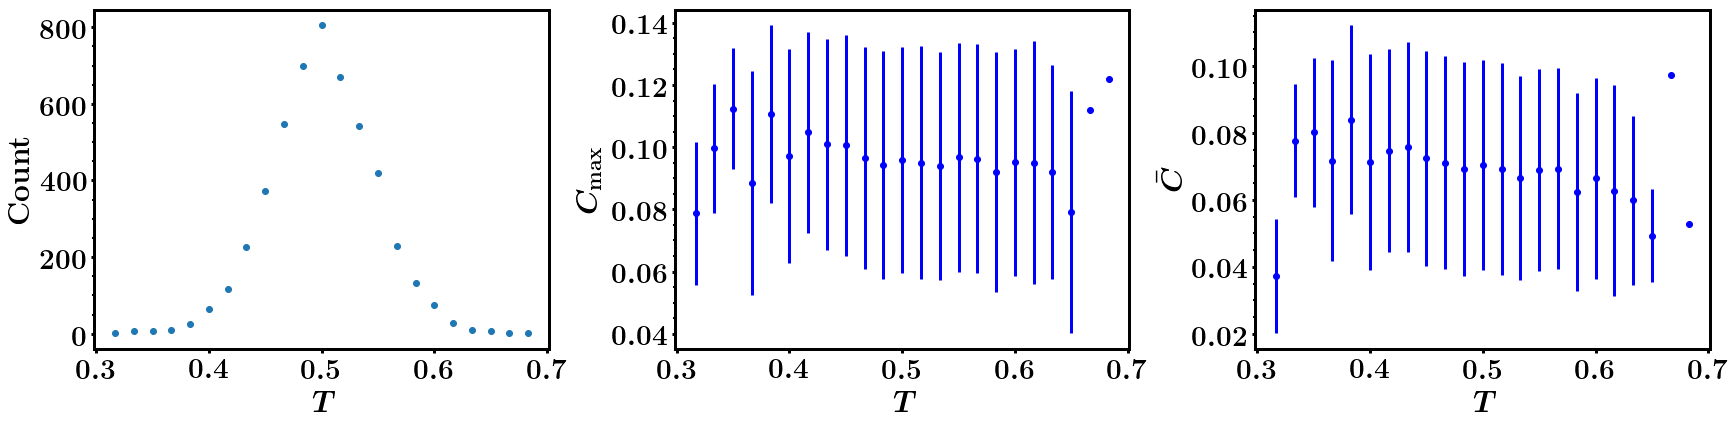
\includegraphics[scale=0.27]{../figs/C_vs_T.png}
	\caption{(Left) Histogram for the triangle index ditribution in the 5000 interaction matrices generated. Values for the max (center) and mean (right) complexities as a function of the triangle index. Dots and bars represent the mean and standard deviation computed over all the matrices with the same value of $T$ \label{C_vs_T}}
\end{figure}

In Figure \ref{C_vs_A} we show the maximum and mean complexity plotted against the normalized algebraic conflict.  No clear correlation can be seen for this balance measure.

\begin{figure}[H]
	\centering
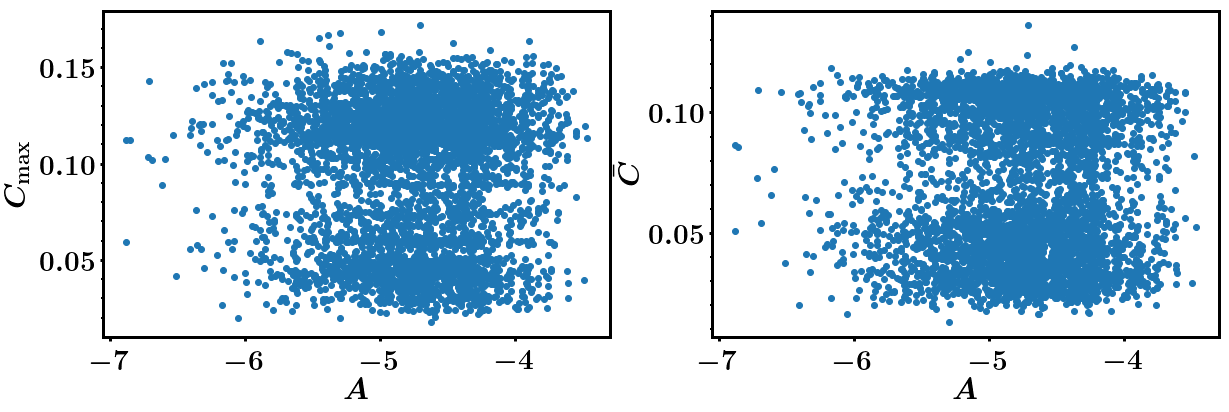
\includegraphics[scale=0.35]{../figs/C_vs_A.png}
	\caption{Max (left) and mean (right) complexities of each realization plotted against the normalized algebraic conflict. \label{C_vs_A}}
\end{figure}


In Figure \ref{C_vs_W} we show the maximum and mean complexity plotted against the walk-based index of balance.  Again, there is not a good correlation using this measure.

\begin{figure}[H]
	\centering
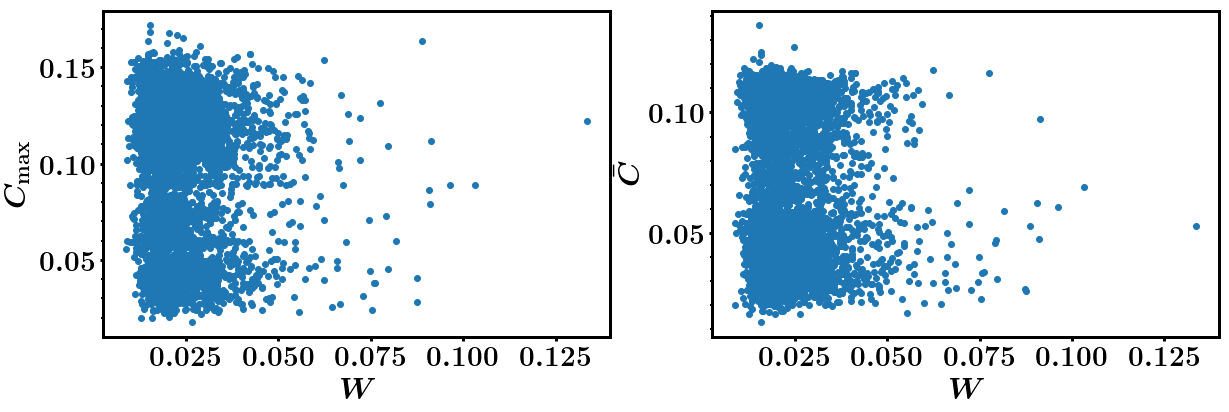
\includegraphics[scale=0.35]{../figs/C_vs_W.png}
	\caption{Max (left) and mean (right) complexities of each realization plotted against the walk-based measure of balance. \label{C_vs_W}}
\end{figure}

\Urlmuskip=0mu plus 1mu\relax
\bibliography{referencias}
\bibliographystyle{ieeetr}


\end{document}